\documentclass[a4paper, 10pt]{article}
% Packages
\usepackage[utf8]{inputenc}  % For Unicode support
\usepackage{amsmath}         % For math symbols
\usepackage{graphicx}        % For including images
\usepackage{hyperref}        % For hyperlinks
\usepackage{graphicx}        % For image rendering
\usepackage{listings}        % For code blocks
\usepackage{sectsty}         % For section font formatting
\usepackage[a4paper, total={7in,9.5in}]{geometry} % For Margins
\usepackage{xcolor}
\usepackage{hyperref}
\usepackage{mathptmx}

% Package Initialization
\graphicspath{{./images/}}

% Formatting
\sectionfont{\fontsize{16}{14}\selectfont}
\hypersetup{
    colorlinks=true,
    linkcolor=blue,
    filecolor=magenta,
    urlcolor=cyan,
}
% Define the style for C++ code
\lstdefinestyle{cpp}{
    language=C++,
    basicstyle=\ttfamily\small,
    keywordstyle=\color{blue},
    stringstyle=\color{red},
    commentstyle=\color{gray},
    morecomment=[l][\color{magenta}]{\#},
    % numbers=left,
    numberstyle=\tiny\color{gray},
    stepnumber=1,
    numbersep=8pt,
    showstringspaces=false,
    breaklines=true,
    % frame=single,
    rulecolor=\color{black},
    backgroundcolor=\color{white},
    tabsize=2,
    captionpos=b
}

% Title, author, date
\title{A Tour of C++}
\author{ksolomon}
\date{\today}

\begin{document}

\maketitle

\begin{abstract}
	Provide an overview on how c++ language is structured and managed in backend. Introduce core language features and concepts on a high-level.
\end{abstract}


%%%%%%%%%%%%%%%%%%%%%%%%%%%%%%%%%%%%%%%%%%%%%%%%%%%%%%%%%%%%
% Chapter 1 - The Basics
%%%%%%%%%%%%%%%%%%%%%%%%%%%%%%%%%%%%%%%%%%%%%%%%%%%%%%%%%%%%

\section{The Basics}
\subsection{Introduction}
\begin{figure}[ht]
	\centering
	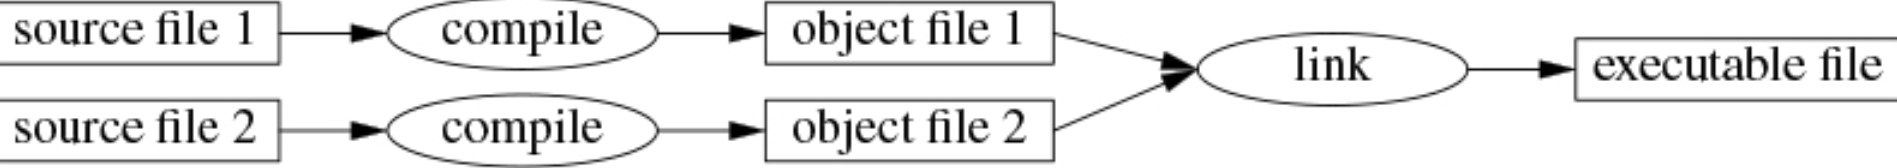
\includegraphics[width=0.7\textwidth]{linker.png}
	\caption{Build Pipeline}
\end{figure}

\subsection{Programs}
ISO standard has 2 types of entities:
\begin{itemize}
	\item Core Language Features (\verb!char, int, for, while!, etc.)
	\item STL Components (\verb!vector, map, cout, getline!, etc.)
\end{itemize}
The STL (Standard Template Library) is (mostly) implemented in C++, providing things like containers, algorithms, etc. which make C++ far more capable as a modern programming language than its predecessor C.
Every C++ program must have exactly one global function: \verb!main() {}!. The return value is treated as the error code. Returning void (nothing) or 0 are treated as a pass. See an example 'Hello World' program below:
\begin{lstlisting}[style=cpp]
import std; // new to C++20 (instead of #include <iostream>)
int main()
{
    std::cout << "Hello World!\n";
    return 0;
}
\end{lstlisting}

Alternatively, if you use the namespace you don't have to explicitly define which namespaces are in scope. However, this basically imports that entire namespace into this translation unit, so 'using' namespaces can cause bloat to binary size.
\begin{lstlisting}[style=cpp]
import std; // new to C++20 (instead of #include <iostream>)
using namespace std;
int main()
{
    cout << "Hello World!\n";
    return 0;
}
\end{lstlisting}

\subsection{Functions}
Declaration: \verb!returnType functionName(argType);!\newline
Defintion: \verb!returnType functionName(argType argName){<implementation>;}!
\newline
While declarations may supply argName, that will be ignored by the compiler, still requiring the function definition to supply the argName. Functions can be standalone, or member functions as part of a larger class. The primary goal of the 'function' is to break code into logical blocks. Appropriate usage of functions make code far more readable and maintainable.\newline
In C++ the compiler can handle something called 'function overloading'. This is where you have multiple permutations/implementations of the same function which take different inputs. With this the user can simply call the function with whatever input types are implemented and the compiler will determine which is the appropriate implementation to use.

\begin{lstlisting}[style=cpp]
void print(int);
void print(double);
void print(string);
//...
// user code each calls appropriate print() function
print(1);
print(2.0);
print('3');
\end{lstlisting}

\subsection{Types, Variables, Arithmetic}
\begin{description}
	\item[Declaration]
	      a statement that introduces an entity into the program and specifies its type.
\end{description}
\begin{description}
	\item[Type]
	      defines a \href{https://en.cppreference.com/w/cpp/language/types}{set of possible values} and a set of possible operations (for given object).
\end{description}
\begin{description}
	\item[Object]
	      memory that holds a value of some defined type.
\end{description}
\begin{description}
	\item[Value]
	      a collection of Bits interpreted according to its type.
\end{description}
\begin{description}
	\item[Variable]
	      a named object.
\end{description}
When performing operations between two different types the result is stored in the type with highest precision (most bits).
e.g.:
\begin{lstlisting}[style=cpp]
double d = 1.0;
int i = 2;
auto res = d + i; // res is a double type (3.0)
\end{lstlisting}
When there are multiple operations on one line the order of operations is as follows (left is hi priority):\newline
\verb!x.y, x->y, x(y), x[y], x<<y, x>>y, x&&y, x||y!

There are multiple ways to initialize variables. All of said methods involve either = or {}. See below for examples:
\begin{lstlisting}[style=cpp]
double d1 = 2.3;
double d2 {2.3};
double d3 = {2.3};
complex<double> z1 = 1; // complex number with double precision scalar input
complex<double> z2 {d1,d2}; // complex number with variable input
complex<double> z3 = {d1,d2}; // = is optional, but maintained for c compatibility
vector<int> v {1,2,3,4,5};
\end{lstlisting}
One main reason to avoid equal (=) assignment is that it can implicitly perform narrowing conversions (which lose information). Examples include int-char and double-int. However, = is preferred when using the \verb!auto! type. \verb!auto! allows the compiler to deduce the type given initial value form at compile time e.g.:
\begin{lstlisting}[style=cpp]
auto b = true; // bool
auto ch = x; // char
auto i = 123; // int
auto d = 1.2; // double
auto z = sqrt(y); // whatever sqrt returns (could be complex<double>)
auto bb {true}; // bool
\end{lstlisting}
\verb!auto! is generally preferred unless:
\begin{itemize}
	\item the variable has a large scope
	\item the type of initializer is non-obvious
	\item we want to explicitly define the precision (e.g. \verb!double! vs \verb!float!)
\end{itemize}
This allows the compiler to perform optimization more effectively and can make code more readable by limiting usage of cumbersome typenames.
\subsection{Scope}
\begin{description}
	\item[Scope]
	      lifetime of the variable/entity, defined by the declaration
	\item[Local]
	      declared in function or lambda. Scope is until the end of the block (defined by {})
	\item[Class]
	      a.k.a. "member" scope. Var is declared within a class, but outside any enum/function/lamba. Scope is within the class open/close {}
	\item[Namespace]
	      Defined in a namespace, but outside any class/function/enum/lambda. Scope is anywhere that namespace is used.
	\item[Global]
	      Defined outside any of above. Available in any translation unit.
\end{description}
An object must be initialized (constructed) before use and it will be destroyed (destructed) at the end of its scope. Attempts to use destructed objects could result in undefined behavior such as use-after-free, stack overflow, etc.
Objects can also be created/destroyed via \verb!malloc()! on the heap by use of \verb!new/delete!.

\subsection{Constants}
\begin{description}
	\item[const]
	      value cannot be changed once set. Can be evaluated at either compile time or runtime.
\end{description}
\begin{description}
	\item[constexpr]
	      function or variable evaluated at compile time. This allows placement into read-only memory (ROM). Exception is that constexpr functions can be called at runtime, but do not generate constexpr output in that case.
\end{description}
\begin{description}
	\item[consteval]
	      a function that can only be used at compile-time. Always generates constexpr output.
\end{description}
\begin{lstlisting}[style=cpp]
    double sum(const vector<double>&); // can read but not modify input argument
    const double s1 = sum(v); // legal. s1 can be calculated at runtime, but not changed thereafter.
    constexpr double s2 = sum(v); // ILLEGAL. sum(v) is not a constant expression/cannot be read-only at compile time.
\end{lstlisting}
For a function to be used in a constant expression (i.e. evaluated at compile-time) it must be defined as \verb!constexpr/consteval!. These functions CANNOT have side-effects, meaning they may only modify local variables.

\subsection{Pointers, Arrays, Reference}
\begin{description}
	\item[Array (v)]
	      collection of data in a contiguously allocated sequence of elements of the same type (0-indexed)
\end{description}
\begin{description}
	\item[Pointer (p)]
	      object that points to another object
\end{description}
\begin{description}
	\item[nullptr:]
	      value of pointers when there is no object available. Attempts to dereference will result in nullptr exception or use after free errors. This is recommended over using the C-style \verb!NULL!, which just aliases 0, and can be confused with an integer.
\end{description}

\begin{figure}[ht]
	\centering
	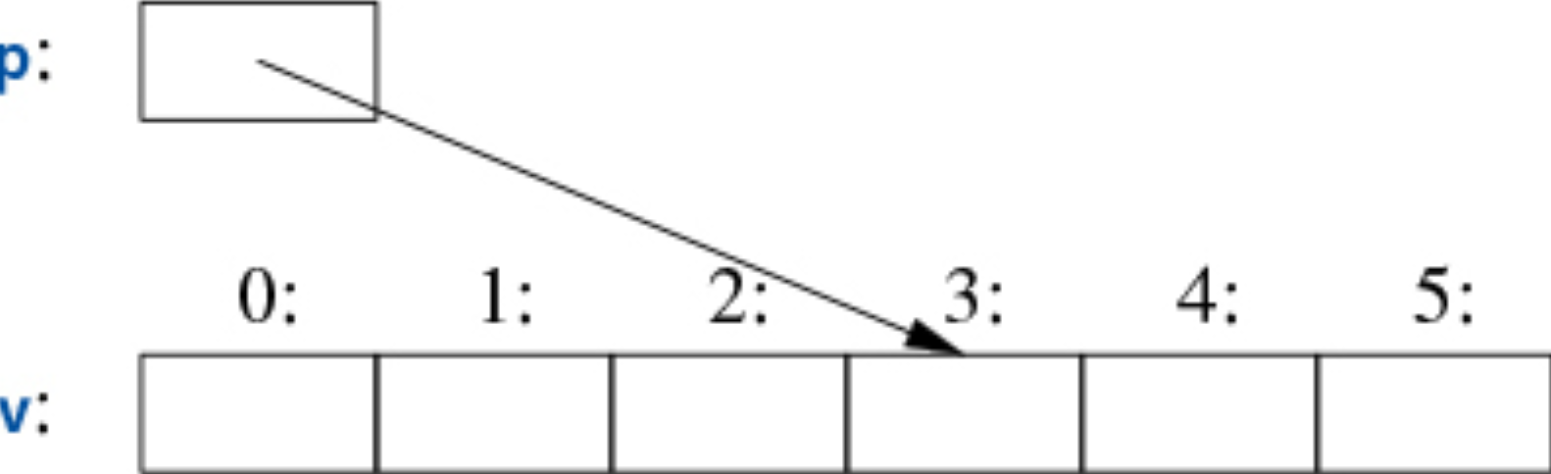
\includegraphics[width=0.5\textwidth]{pointer.png}
	\caption{char* p = \&v[3]}
\end{figure}

\begin{lstlisting}[style=cpp]
    char v[6]; // array of 6 characters
    char* p; // ptr to character
    char* p = &v[3]; // p points to v's 4th element
    char x = *p; // x is the character that p points to (aka same as v[3])
\end{lstlisting}
For loops are a typical way to iterate through arrays:
\begin{lstlisting}[style=cpp]
    int v[] = {0,1,2,3,4,5,6,7,8,9};
    for(auto i = 0; i < 10; i ++){;}
    for(auto x : v){;}
    for(auto x : {'a','b','c'}){;}
    for(auto& x : v){++x;} // since this give a reference to x you can modify in-place
\end{lstlisting}
References are especially useful for function arguments since it allows the function to mutate the
argument without copying the whole of the argument(s) onto the stack. If we dont want to modify the
contents then use const modifier
\begin{lstlisting}[style=cpp]
    double sum(const vector<double>&){}
\end{lstlisting}

\subsection{Tests (Conditionals)}
These check to see if values are some form of equivalent or less than, greater than one another.
Common structures include \verb!if()! statements and \verb!switch/case! statements.
\begin{lstlisting}[style=cpp]
    if(a < b){}
    else if(a > b){} // where there is an elseif statement it is good practice to always have else case
    else {}

    switch(ch) {
        case 'a':
            // if ch == 'a' it will trigger code here
        case 'b':
            // 'a' case falls-down and also runs code here since there was no 'break' after case 'a'
            // if ch == 'b' then only this section is run, above code in case 'a' section is not run.
            break;
        case 'c':
            // if ch == 'c' it will trigger code here
            break;
        default:
            // if ch == anything but 'a'-'c' it will trigger code in the default case
    }



\end{lstlisting}

\subsection{Advice for Getting Started}
\begin{enumerate}
	\item Dont panic, you don't need to know all the details to write good code.
	\item Don't use built-in features exclusively, STL is powerful.
	\item Import libraries when possible.
\end{enumerate}


%%%%%%%%%%%%%%%%%%%%%%%%%%%%%%%%%%%%%%%%%%%%%%%%%%%%%%%%%%%%
% Chapter 2 - User-Defined Types
%%%%%%%%%%%%%%%%%%%%%%%%%%%%%%%%%%%%%%%%%%%%%%%%%%%%%%%%%%%%

\section{The Basics}
\begin{description}
	\item[Built-In Types:]
	      types which can be built entirely from the fundamental types, the \verb!const! modifier, and declarator operators.
\end{description}
\subsection{Struct}
\begin{description}
	\item[struct]
	      organized/grouped set of variable types that collectively make some larger concept.
\end{description}
\begin{lstlisting}[style=cpp]
    // Defintion
    struct Vector {
        double* elem;
        int sz;
    }

    // Usage
    Vector v;
    int size = 10;
    v.elem = new double[size];
    if(v.elem != nullptr) // this would happen if there is not room in memory to allocate 10 elements
        v.sz = size;
\end{lstlisting}
\subsection{Classes}
\begin{description}
	\item[Class:]
	      similar to a struct in that it organizes data and represents some greater entity/concept than just a variable, however a struct has members public by default. A class can hide private implementation. Constructors/Destructors are also a concept unique to classes.
\end{description}
\begin{description}
	\item[Vector:]
	      a handle containing a ptr to elements and the number of elements (sz)
\end{description}
\begin{lstlisting}[style=cpp]
class Vector {
  public:
    Vector(int s) :elem{new double[s]}, sz{s} {} // Constructor is same name as class with no return type
    double& operator[](int i) { return elem[i];} // Operator overloading for dereferencing *elem;
    int size() {return sz;} // access function to read (but not have write-access to) private member variable
  private:
    double* elem;
    int sz;
}
\end{lstlisting}

\begin{figure}[ht]
	\centering
	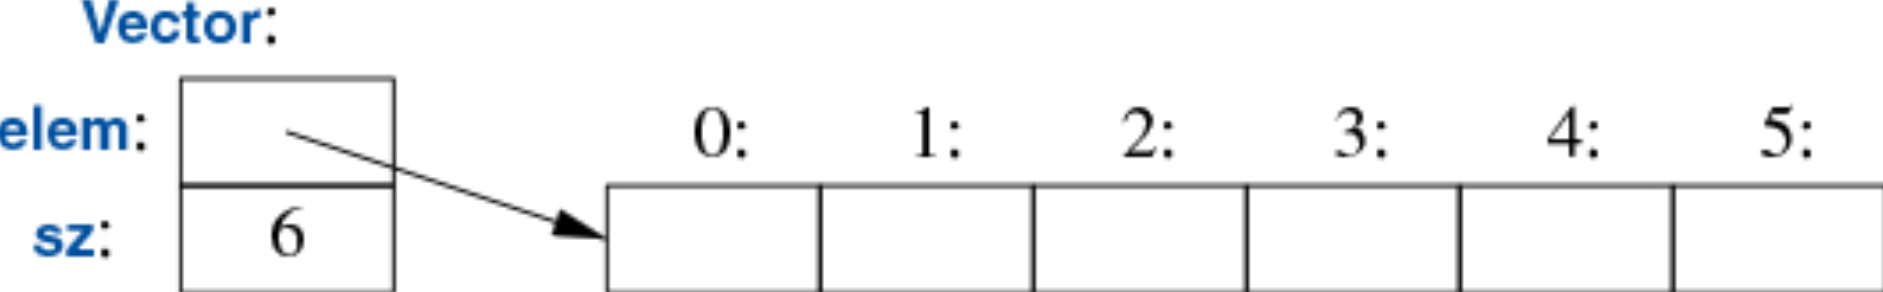
\includegraphics[width=0.5\textwidth]{vector.png}
	\caption{Simple representation of a Vector}
\end{figure}

In our example vector class we use an initializer list constructor \verb!:elem{new double[s]}, sz{s}!. This defines elem with a pointer to s elements of type double. Then we initialize sz to s.

\subsection{Enum}
\begin{description}
	\item[Enum:]
	      User-defined types that have a fixed set of possible values (integer only).
\end{description}
By default enums have assignment, initialization, and comparison operators.
\begin{lstlisting}[style=cpp]
// OK
enum class Color {RED, GREEN, BLUE};
enum class TrafficLight {RED, YELLOW, GREEN};
enum names {BETHANY, TAYLOR, KARL}; // C-Style enum is just an integer wrapper
Color col = Color::RED;
TrafficLight tl = TrafficLight::RED;

int i = Color::RED; // ERROR: RED is not an int.
int i = int(Color::RED); // Legal type cast
int i = names::BETHANY; // Legal C-style
Color c = 2; // ERROR: 2 is not a Color
names n = 1; // Legal: C-style maps to names::TAYLOR
Color c {2}; // Legal
\end{lstlisting}

\subsection{Union}
\begin{description}
	\item[Union:]
	      All members are allocated at the same memory address.
\end{description}
\begin{description}
	\item[Variant:]
	      stores a value of one of a set of alternative types.
\end{description}
Unions only occupy as much memory as the largest member. Unions are typically used to implement a single variable that can contain multiple different types of data. This way, depending on the context, the variable can be viewed/manipulated differently without dealing with messy type casting.
\verb!Variant! types were introduced in C++17. These can effectively replace unions in many cases, and are the preferred choice in C++17 and later.
\begin{lstlisting}[style=cpp]
    struct Entry {
        string name;
        variant<Node*, int> v; // can represent the variable as EITHER Node* OR int.
    }
    void f(Entry* pe) {
        if(holds_alternative<int>(pe->v)) {
            cout << get<int>(pe->v) << endl;
        }
    }
\end{lstlisting}


%%%%%%%%%%%%%%%%%%%%%%%%%%%%%%%%%%%%%%%%%%%%%%%%%%%%%%%%%%%%
% Chapter 3 - Modularity
%%%%%%%%%%%%%%%%%%%%%%%%%%%%%%%%%%%%%%%%%%%%%%%%%%%%%%%%%%%%

\section{Modularity}
\subsection{Introduction}
Crutial for modular code to separate interface from implementation.
\begin{description}
	\item[Declaration:]
	      interface - everything that is needed to use a function.
\end{description}
\begin{description}
	\item[Definition:]
	      implementation - how the function achieves promised interface.
\end{description}
There can be multiple declarations, but only one definition per entity.
\subsection{Separate Compilation}
In order to achieve modular code it is important to separate code into logical units. Each .c/.cpp file that contains implementaion is compiled separately into its own 'translation unit'. These translation units are linked together with the linker after all of the units are compiled. In order for source code to reference code in a different translation unit the source must either include the header file which defines the interface, or it must import the module which defines a library containing the target code. While the header file route is most popular currently, with the addition of import functionality in C++20 import is now preferred.
\paragraph {Headers}
\begin{figure}[ht]
	\centering
	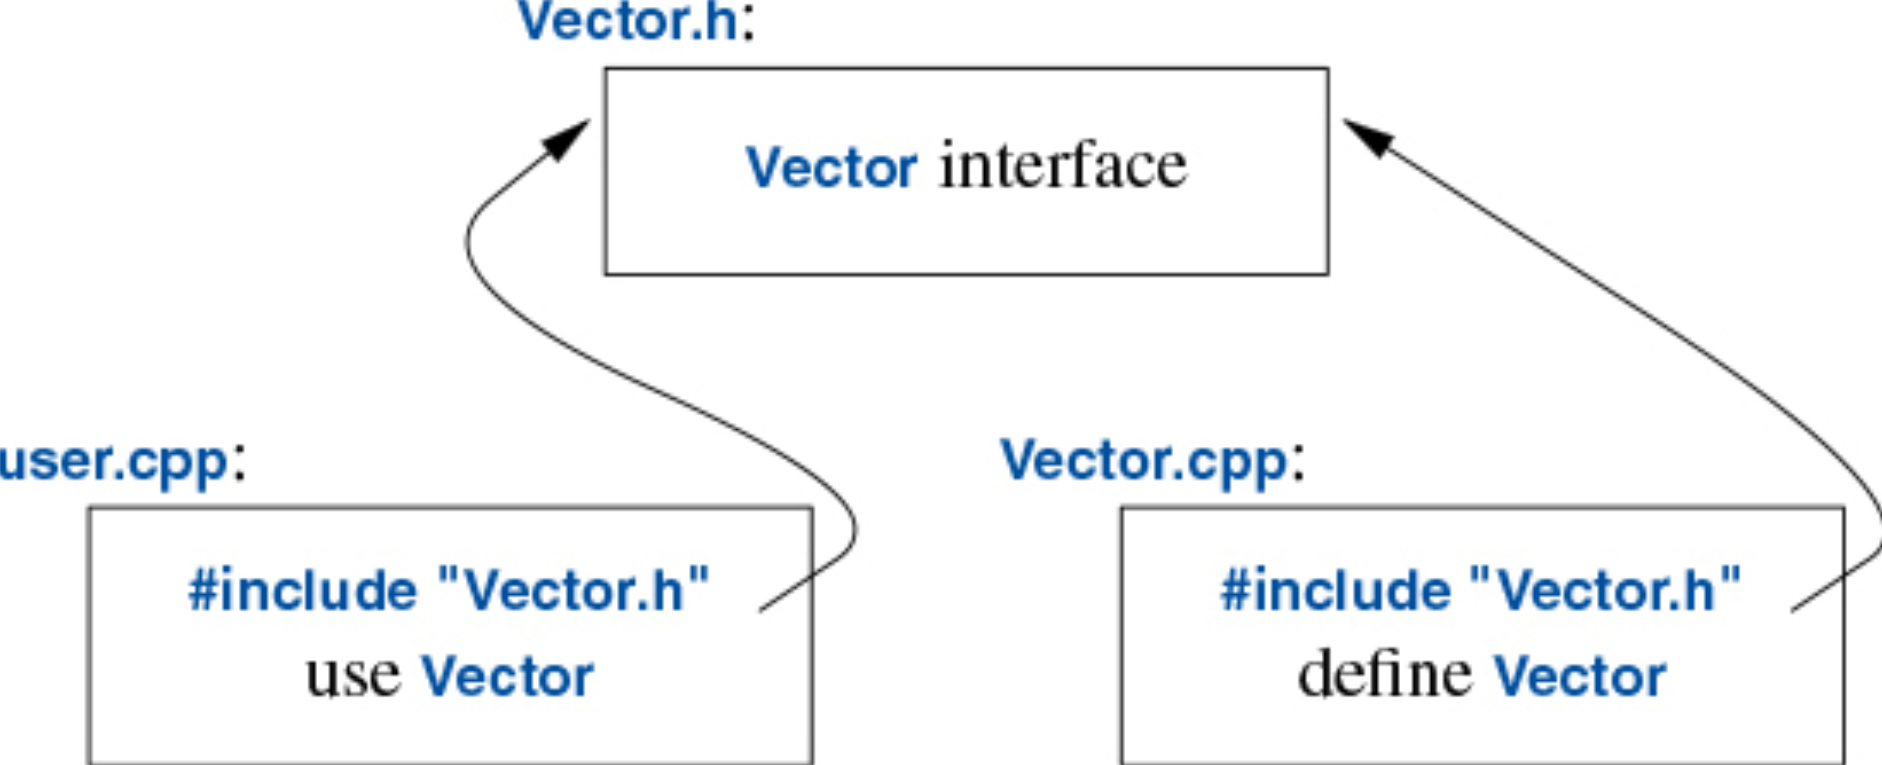
\includegraphics[width=0.4\textwidth]{images/header.png}
	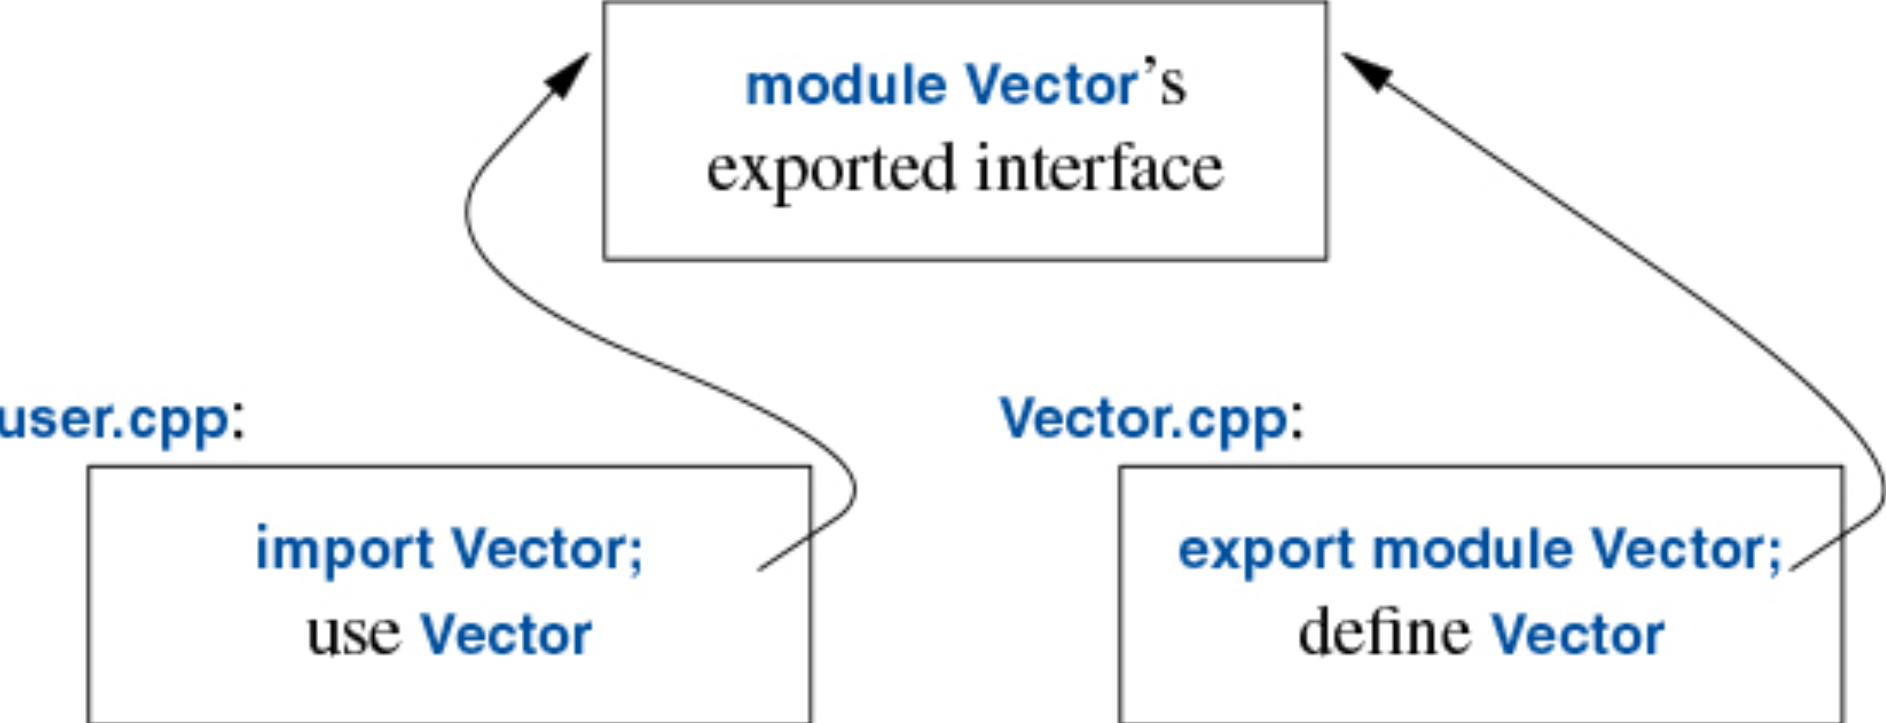
\includegraphics[width=0.4\textwidth]{images/module.png}
	\caption{Graphical header vs module reference flow.}
\end{figure}
The best mental-model is to consider a program as a set of modules, each of which is a translation unit responsible for its own concept. One major disadvantage of the C-style modules using include directives is that each include statement completely injects/copies the contents of said header file into the translation unit (source/.c/.cpp) file. This means that if N files import x.h then x.h's text is copied into N files. This can create serious bloat and increase compile time. Another disadvantage is that the order of includes matters in the source file. Consider the following legitimate example:
\begin{lstlisting}[style=cpp]
#include 'a.h'
#include 'b.h'
doStuff(); // Compiler Error - Object not found

// vs

#include 'b.h'
#include 'a.h'
doStuff(); // Pass
\end{lstlisting}
\paragraph{Modules}
Consider the below usage of \verb!import!. Here we show that we can both \verb!import! and \verb!#include! in the same file. The main advantage of using import over include is that we can avoid excessive code copying from include. Only the units which are 'exported' will be included in the translation unit. Additionally, the compiler will check for the existence of the module and prevent redundant imports. This should considerably improve maintainability and compile times. This can prevent unnecessary complication of source code into .hpp and .cpp files since we can just selectively export specific entities in the .cpp.

\begin{lstlisting}[style=cpp]
export module Vector;
export class Vector{
    public:
    Vector(int s);
    double& operator[](int i);
    int size();
    private:

}
\end{lstlisting}
\subsection{Namespaces}
Namespaces allow you to use class/function/variable names that are present in different namespaces differently. E.g. you can create your own implementation of C++ STL libraries (e.g. vector, printf, etc.). The simplest way to access an entity in a different namespace is to use the \verb!::! operator (e.g. \verb!std::vector!). To gain access to all names in any namespace use \verb!using namespace <namespace>;!. This is has consequences if used carelessly since it can use names that you may not be aware of and intend to build yourself. These are primarily used to organize libraries.
\subsection{Arguments}
Key concerns are:
\begin{itemize}
	\item pass by value or reference
	\item const or mutable
	\item side-effects (e.g. if an object is moved then previous reference is invalid).
\end{itemize}
Default behavior is pass-by-value. However, compiler optimization can implicitly modify to pass-by-reference. It is generally faster to pass-by-value when the \verb!sizeof(object) < 4*sizeof(void*)!. Use \verb!const! modifier if we want to pass by reference, but don't need to actually modify the value
\lstinputlisting[style=cpp] {sources/arguments.sumTwoVectors.cpp}
It is common for arguments to have a default value. An example of such usage can be seen here:\newline
\verb!void print(int value, int base = 10); // 10 is default for base!
\paragraph{Return} by reference only when returning something that is not local to the caller. Anything local to the caller will be destroyed when the function returns. Most compilers should throw this error at compile-time. If a large object is created inside a function and needs to be returned to the caller it can be achieved by generating a \verb!move! constructor for the object. It is \textit{possible} that even without explicitly defining a move constructor that the compiler can optimize away the copy and implicitly perform a move. This is called \textit{copy elision}. See below for an example in modern copy elision in practice:
\lstinputlisting[style=cpp] {sources/arguments.copyElision.cpp}
\paragraph{Deduction} of return type is possible by returning \verb!auto!. This is especially valuable for generics and lambdas. It is possible to display the return type after the function handle and arguments like so:
\begin{lstlisting}[style=cpp]
auto sqrt(double); // deduction
auto sqrt(double) -> double; // suffix-return type
\end{lstlisting}

\pagebreak
\section{Errors}

\pagebreak
\section{Classes}
\subsection{Concrete Types}
Behave just like built-in types e.g. complex numbers and infinite-precision integers. Representation is part of its definition. Typically these are used for types which don't change often and depend on private members.
Upside:
\begin{itemize}
	\item Easy to place on stack/heap and in other objects
	\item Can refer to objects directly, not just via reference
	\item Initialize objects immediately and completely in constructor
	\item Copy/move easily
\end{itemize}
Downside:
\begin{itemize}
	\item Any change causes recompilation.
\end{itemize}
\paragraph{Arithmetic} types are a classic example of concrete types, for example complex numbers.
\subsection{Abstract Types}
\subsection{Virtual Functions}
\subsection{Class Hierarchies}

% References
\begin{thebibliography}{9}
	\bibitem{latex}
	Leslie Lamport.
	\textit{A Tour of C++: 3rd Edition}.
	Bjarne Stroustrup, 2022.

\end{thebibliography}

\end{document}
